
%% setup
\documentclass[a4paper, 11pt, openany]{book}
\emergencystretch 3em % avoid overfulls in right margin
\usepackage[a4paper]{geometry}
\geometry{lmargin=2.5cm,rmargin=2.5cm,tmargin=2.5cm,bmargin=2.5cm}

%% fonts
\usepackage{ebgaramond} % serif font
\usepackage{lato} % sans serif font
\usepackage{sectsty} % for setting frontmatter and section headings to sans serif
\allsectionsfont{\raggedright\normalfont\lato\bfseries} % ^ bold + sans serif section headings; aligned left

%% define metadata
\def \documenttitle {Specification of `normal' wind turbine operating behaviour for rapid anomaly detection: through the use of machine learning algorithms}
\def \authorname {Nithiya M Streethran}
\def \keywords {wind turbine, classification algorithm, SCADA, fault detection, condition monitoring}
\def \licenseurl {https://creativecommons.org/licenses/by/4.0/}
\def \documentdate {25 August, 2017}
\def \programme {MSc in Renewable Energy Engineering}

%% metadata and hyperlink setup
\title{\textbf\documenttitle}
\author{\authorname}
\date{\documentdate}
\usepackage[hidelinks]{hyperref}
\usepackage{hyperxmp}
\hypersetup{
    colorlinks=true,
    urlcolor=blue,
    linkcolor=blue,
    citecolor=blue,
    pdfauthor={\authorname},
    pdftitle={\documenttitle},
    pdfkeywords={\keywords},
    pdflicenseurl=\licenseurl,
    pdfproducer={xelatex}
}
\urlstyle{same} % don't use monospace font for urls

%% header and footer
\usepackage{fancyhdr} % for header and footer
\pagestyle{fancy}
\fancypagestyle{plain}{
	\fancyhf{}
	\renewcommand{\headrulewidth}{0pt}
	\fancyfoot[C]{\thepage}
}
\fancyhf{} % sets both header and footer to nothing
\renewcommand{\headrulewidth}{0pt} % remove horizontal line from header
\fancyfoot[RO,LE]{\thepage} % page number
\fancyfoot[RE,LO]{\textit\programme}
\makeatletter
\fancyhead[RE]{\authorname} % name
\makeatother
\fancyhead[LO]{\textit{\nouppercase{\leftmark}}} % Chapter title
\renewcommand{\chaptermark}[1]{\markboth{#1}{}}

%% bibliography
\usepackage[backend=biber,style=ieee,uniquename=init,giveninits,urldate=long]{biblatex}
\usepackage{xpatch} % to remove empty parentheses if year not provided for @online
\xpatchbibdriver{online}
{\printtext[parens]{\usebibmacro{date}}}
{\iffieldundef{year}{}{\printtext[parens]{\usebibmacro{date}}}}
{}{}
\renewbibmacro*{doi+eprint+url}{%
% if DOI is not present, print eprint; if eprint is not present, print URL
	\printfield{doi}%
	\newunit\newblock%
	\newunit\newblock%
	\iffieldundef{doi}{%
		\usebibmacro{eprint}%
		\iffieldundef{eprint}{%
			\usebibmacro{url+urldate}}}%
	{}%
}
\addbibresource{references.bib} % bibliography file

%% contents and floats
\renewcommand*\contentsname{Table of Contents}
\usepackage[nottoc,notbib]{tocbibind} % adding lists to the toc
\usepackage[font=small,labelfont=bf]{caption} % caption font size = small
\usepackage{floatrow} % to modify float settings 
\floatsetup[table]{capposition=top} % force table captions on top
\usepackage{graphicx}
\graphicspath{{../images/}}
% set default figure placement
\makeatletter
\def\fps@figure{!htb}
\makeatother
\usepackage{pdflscape} % for changing page orientation

%%%
\begin{document}

    \frontmatter
    \begin{titlepage}
        \hspace{0pt} % vertical centering
        \vfill % ^
        \centering % horizontal centering
        \huge\textbf\documenttitle
        \\[2cm]
        \Large Dissertation for the Degree of \programme
        \\
        Heriot-Watt University
        \\[2cm]
        \authorname \textsuperscript{\,1, }*
        \\[.3cm]
        Supervisors: Dr Nick Bennett \textsuperscript{2} and Dr Iain Dinwoodie \textsuperscript{3}
        \\[.3cm]
        \large
        \textsuperscript{1, 2} School of Engineering and Physical Sciences, Heriot-Watt University, Edinburgh EH14 4AS, United Kingdom
        \\
        \textsuperscript{3} Natural Power Consultants, Ltd., Stirling FK7 7XE, United Kingdom
        \\[.3cm]
        * Email: nmstreethran@gmail.com
        \\[2cm]
        \Large
        Submitted on \documentdate
        \\[.3cm]
        Reformatted and recompiled on \today
        \vfill % vertical centering
        \hspace{0pt} % ^
    \end{titlepage}
    
\chapter{Abstract}

Maximising the economic effectiveness of a wind farm is essential in making wind a more economic source of energy. This effectiveness can be increased through the reduction of operation and maintenance costs, which can be achieved through continuously monitoring the condition of wind turbines. An alternative to expensive condition monitoring systems, which can be uneconomical especially for older wind turbines, is to implement classification algorithms on supervisory control and data acquisition (SCADA) signals, which are collected in most wind turbines. Several publications were reviewed, which were all found to use separate algorithms to predict specific faults in advance. In reality, wind turbines tend to have multiple faults which may happen simultaneously and have correlations with one another. This project focusses on developing a methodology to predict multiple wind turbine faults in advance simultaneously by implementing classification algorithms on SCADA signals for a wind farm with 25 turbines rated at 2,500 kW, spanning a period of 30 months. The data, which included measurements of wind speed, active power and pitch angle, was labelled using corresponding downtime data to detect normal behaviour, faults and varying timescales before a fault occurs. Three different classification algorithms, namely decision trees, random forests and k nearest neighbours were tested using imbalanced and balanced training data, initially to optimise a number of hyperparameters. The random forest classifier produced the best results. Upon conducting a more detailed analysis on the performance of specific faults, it was found that the classifier was unable to detect the varying timescales before a fault with accuracy comparable to that of normal or faulty behaviour. This could have been due to the SCADA data, which are used as features, being unsuitable for detecting the faults, and there is potential to improve this by balancing only these classes.
\\[.5cm]
\noindent\textbf{\textit{Keywords:}} \keywords{}

    \tableofcontents
    \listoffigures
    \listoftables

    \mainmatter
    
\chapter{Introduction}\label{c1}

\section{Background}

There is a need to increase the economic effectiveness of wind turbines, which refers to the cost to run them relative to the electricity generation, or revenue \cite{Kim12,Leahy16}. Increasing this effectiveness lowers the payback period of new wind turbines or farms, thus making wind a more economic clean energy source, attracting governments and private organisations to make more investments in wind projects \cite{Kim12}. It can, however, be decreased due to major component failure, frequent downtime, turbine degradation and age, which in turn increase the operation and maintenance cost and decrease the energy generation efficiency of wind turbines \cite{Kim12,Diens16}. There are difficulties and high costs involved in carrying out maintenance on wind turbines, especially for ones that operate in extreme and remote conditions, such as offshore wind farms, where the turbines tend to also exist in larger numbers \cite{Diens16,Tautz17}.

Condition-based monitoring systems that continuously monitor wind turbine states increase this effectiveness by significantly reducing the maintenance costs, reportedly by 20\,\% to 25\.\%, as it prevents unscheduled maintenance \cite{Leahy16}. According to the Electric Power Research Institute, reactive maintenance, which refers to running the turbine until it reaches failure, has the highest cost, followed by preventive or scheduled maintenance, which is reported to cost 24\,\% less \cite{Wind15}. Meanwhile, condition-based or predictive maintenance, which prevents catastrophic failure, \cite{Kim12} is reported to save 47\,\% of the cost of reactive maintenance, \cite{Wind15} which makes it the most cost-effective and preferred approach. Condition-based monitoring technologies include sensor-based oil and vibration analysis, which are useful for checking the oil for properties such as temperature, and rotating equipment respectively \cite{Garci12}. These technologies, however, tend to put emphasis on the more expensive parts of a wind turbine such as the gearbox \cite{Godwi13} due to the high costs involved in the installation of these sensors \cite{Leahy16,Garci12}. These systems, which can be purchased from the turbine manufacturer, are usually pre-installed in offshore wind turbines due to the harsh environments in which they operate. However, they can be expensive \cite{Tautz17} and uneconomical, especially for older wind turbines in onshore wind farms, whose outputs are often less than that of an offshore wind farm.

An alternative would be to use SCADA-based analysis, where the only cost involved would be computational and expensive sensors are not required \cite{Tautz17,Leahy16}. A SCADA system, which stands for supervisory control and data acquisition, found pre-installed in most utility-scale wind turbines, collects data using numerous sensors at the controllers with usually 10-minute resolution \cite{Tautz17,Yang14}, of various parameters of the wind turbine, such as wind speed, active power, bearing temperature and voltage \cite{Leahy16}. Power curve analysis can be done using this data, but this analysis only detects wind turbine underperformance \cite{Gill12}. Meanwhile, implementing machine learning algorithms on SCADA signals to classify them as having either normal or anomalous behaviour, has the ability to predict faults in advance. This has been demonstrated in a number of publications.

Kusiak and Li \cite{Kusia11} investigated predicting a specific fault, which is diverter malfunction. 3 months' worth of SCADA data of four wind turbines were used and the corresponding status and fault codes were integrated into this data to be labelled to differentiate between normal and fault points. To prevent bias in prediction in machine learning, the labelled data is sampled at random, ensuring the number of samples with a fault code is comparable to the number of normal samples. Four classification algorithms, namely neural networks, boosting tree, support vector machines, and classification and regression trees were trained using two-thirds of this data which was randomly selected. The boosting tree, which was found to have the highest accuracy of 70\,\% for predicting specific faults, was investigated further. The accuracy of predicting a specific fault at the time of fault was 70\,\%, which decreased to 49\,\% for predicting it 1 hour in advance. Only one specific fault was the focus of this methodology and in reality, wind turbines could have many faults in different components and structures, which may all have some form of correlation between one other.

Godwin and Matthews \cite{Godwi13} focussed on wind turbine pitch control faults using a classifier called the RIPPER algorithm. They used 28 months' worth of SCADA data containing wind speeds, pitch motor torques and pitch angles, of eight wind turbines known to have had pitch problems in the past. The classes used were normal, potential fault and recognised fault. Using maintenance logs, data up to 48 hours in advance was classed as recognised fault, data in advance of this with corresponding SCADA alarm logs indicating pitch problems was classed as potential fault, and the remaining unclassed data was classed as normal. Random sampling was performed here as well to balance the classes and prevent bias. The data of four turbines were used to train the RIPPER algorithm, and the remaining four used for testing. The analysis was done using the entire 28 months of data as well as 24, 20, 16, 12, 8 and 4 months of data to find out how the amount of data affects the accuracy of classification. Using the entire 28 months of data was found to produce the most accurate classifier, with a mean accuracy of 85\,\%. Looking at the results in more depth, it was found that the classifier had F1 scores, which is an accuracy measure that accounts for true and false positives and negatives, of 79\,\%, 100\,\% and 78\,\% in classifying normal, potential fault and recognised fault data respectively. Although the results are an improvement to Kusiak and Li \cite{Kusia11}, this methodology similarly focussed on only one fault.

Leahy et al. \cite{Leahy16} used a specific fault prediction approach, implementing a support vector machine classifier from scikit-learn's LibSVM. They used SCADA data from a single 3 MW wind turbine spanning 11 months with status and warning codes. The labelling was done such that data with codes corresponding to the turbine in operation, low and storm wind speeds represent normal conditions and codes corresponding to each specific fault to represent faulty conditions. Data preceding these fault points by 10 minutes and 60 minutes were also labelled as faults in separate sets and the effects of using these different time scales to predict faults were investigated. For data identified as normal, filters were applied to remove curtailment and anomalous points. The classifier's hyperparameters were optimised using randomised grid search and validated using ten-fold cross-validation, and the classes were balanced using class weights. Separate binary classifiers were trained to detect each specific type of fault, which were faults in air cooling, excitation, generator heating, feeding and mains failure. The prediction of generator heating faults 10 minutes in advance had the best results, with F1 scores of 71\,\% and 100\,\% using balanced and imbalanced training data respectively. This increase in score using imbalanced data was attributed to the test set having very few instances with the fault class relative to normal data. The same fault, when predicted 60 minutes in advance, had F1 scores of 17\,\% and 100\,\% using imbalanced and balanced training data respectively. Although the score is perfect and it demonstrates the effects of using balanced datasets, the classification again is done separately for each specific fault and it performed poorly on other faults. For instance, detecting excitation faults 10 and 60 minutes in advance using balanced training data only yielded F1 scores of 8\,\% and 27\,\% respectively.

This project will therefore focus on integrating the ability to predict multiple faults at different time scales simultaneously.

\section{Objectives}

The first objective of this project is to implement a classification algorithm on wind turbine SCADA signals to identify underperforming turbines. This involves setting-up the machine learning environment, processing operational data and reporting initial results obtained through implementing a classification algorithm on the data.

The second objective is to create an effective methodology for the integration of failures and to present and interpret results. This includes labelling the data such that each specific fault can be differentiated, evaluating the performances of several classification algorithms to find the most suitable classifier, identifying limitations and suggesting improvements to the method and how it can be adapted for use in industry.

\section{Outline}

Chapter~\ref{c2} will describe in detail the tools and datasets used, how the data was processed and labelled and the classification methods and performance metrics used. In Chapter~\ref{c3}, a detailed description of the results obtained is presented, followed by a discussion of these results and limitations of this methodology in Chapter~\ref{c4}. In Chapter~\ref{c5}, conclusions are drawn and possible areas for future work are recommended.

    
\chapter{Methodology}

\section{Tools and datasets}

This project requires a computer with Python Programming Language \cite{Welco} and essential libraries installed for data processing. The computer used has a dual core processor with 2.8 GHz maximum clock speed and 4 GB RAM. Additionally, the open source scikit-learn library \cite{Pedre11} is used for machine learning. The datasets used are that of a wind farm comprised of 25 turbines with a rated power of 2,500 kW covering a period of 30 months starting 1st November 2014, downloaded from Natural Power’s database in CSV format. The first dataset is wind turbine SCADA signals timestamped with a resolution of 10 minutes, with a total file size of 452 MB, and the other dataset is corresponding downtime data for the same period, with a total file size of 4 MB. In the interests of Natural Power, the location of the wind farm and turbine model will not be disclosed in this report.

\section{Data processing}

The SCADA data has 17 fields, summarised in Table~\ref{t1}. Fields highlighted in green are average measurements recorded over each 10-minute period. Since these highlighted fields are properties of the turbines or describe its performance, they can be used as features in machine learning. Each turbine has two nacelle anemometers and wind vanes; one is used to control the turbine, and the other to monitor the first. The measurements from the anemometer and wind vane used to control the turbine are recorded again as \texttt{ws\_av} and \texttt{wd\_av}, with the latter taking into account the nacelle position. Using only \texttt{ws\_av} and \texttt{wd\_av} for wind speed and wind direction, the number of features that are available for machine learning is 10.

\begin{table}
    \centering
    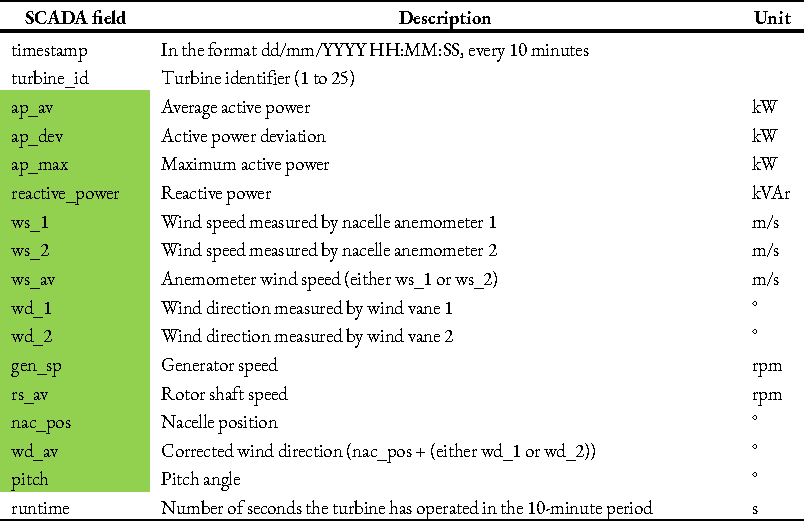
\includegraphics{t1.pdf}
    \caption{\label{t1}Summary of SCADA fields for the SCADA data used in this project. The fields include timestamps with a resolution of 10 minutes, average active power, wind speed, pitch and runtime. The fields that contain measurements averaged over the 10-minute period are highlighted in green. These measurements can be used as features in machine learning as they are turbine properties.}
\end{table}

The downtime data consists of fields summarised in Table~\ref{t2}. Each row of downtime data consists of the start and end timestamps of the downtime event, downtime categories, workorders and alarms. Downtime categories, which are turbine, environmental, grid, infrastructure and availability categories, describes the turbine’s condition or cause of downtime when the maintenance work was undertaken. Each condition within each downtime category is represented by a unique identifier in the dataset. A separate spreadsheet accompanying the dataset list what each identifier stands for. All quantities in the downtime data, except the alarms, are supervised (i.e., the data recordings are input and monitored by maintenance professionals).

\begin{table}
    \centering
    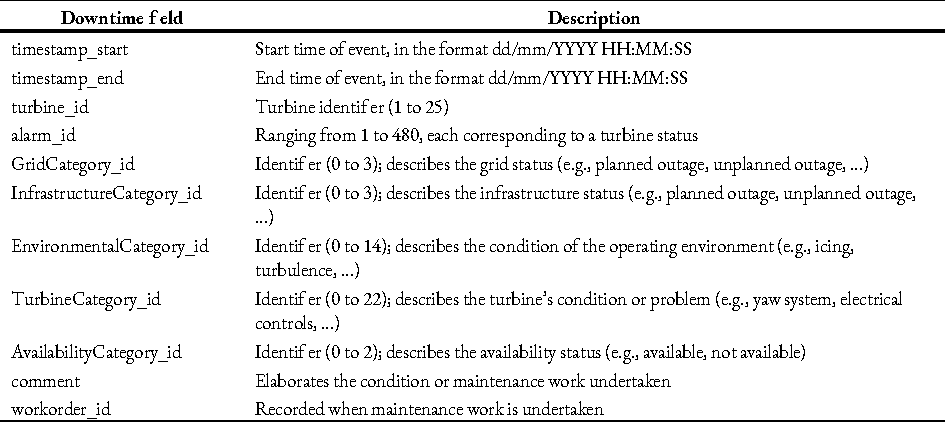
\includegraphics{t2.pdf}
    \caption{\label{t2}Summary of fields for the downtime data used in this project. The fields include start and end timestamps for the downtime event, downtime categories, workorders and alarms.}
\end{table}

Each row of SCADA data requires a class which describes the state of the turbine. The chosen classes are `normal' for normal behaviour, and `faulty' to signify a fault. As the aim is to predict faults in advance, a category of classes, called `before fault' will also be used. To automate the labelling process, the SCADA data can be merged with the downtime data, which has turbine categories, listed in Table~\ref{t3}, that can be used to label faults. Some of these turbine categories, such as `OK' and `scheduled maintenance', do not indicate a fault in the turbine, and `other' does not specify the condition. Therefore, only the turbine categories which indicate faults, highlighted in green, are used to class the SCADA data. Prior to merging the two datasets, the downtime data is restructured such that it has the same 10-minute resolution as the SCADA data. The SCADA data was also found to have missing rows of data. Empty data rows with only the timestamp corresponding to the missing rows were added to rectify this. Once they are merged, 14 separate labels, or columns, are added for each specific fault, which will allow for the different faults to be distinguished. The rows with a fault category are classed as `faulty' in the corresponding column.

\begin{table}
    \centering
    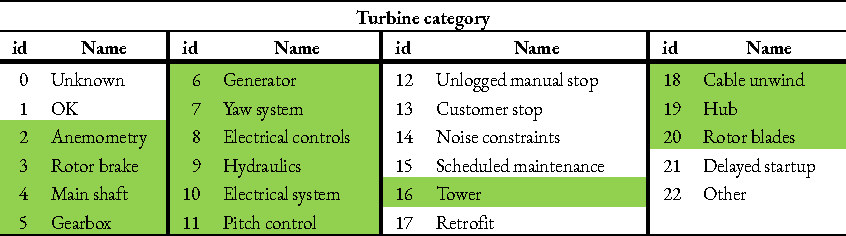
\includegraphics{t3.pdf}
    \caption{\label{t3}List of turbine categories in the wind farm downtime data. The categories used as the different faults for labelling are highlighted in green. The others do not indicate a fault.}
\end{table}

To summarise the machine learning terminology used, features refer to SCADA fields which are turbine properties, labels refer to turbine categories or type of fault, and classes refer to the state of the turbine (e.g., `normal' or `faulty') for each row of data at each label. The features and labels will be fit to a classifier for training as arrays X of size [rows, 10] and Y of size [rows, 14] respectively, where rows refer to the number of rows in the training data.

To predict faults for each label, rows with timestamps up to 48 hours in advance of a `faulty' row are classed at 6-hour intervals (i.e., up to X hours before a fault, where X = 6, 12, …, 48). The reasons for having classes of 6-hour intervals for fault detection rather than a single class is to allow action to be taken appropriate to the time before fault. For example, if it is predicted that the wind turbine could have a fault in six hours or less, it could be switched off to prevent further damage from occurring. 48 hours is enough time for maintenance professionals to travel to site and carry out inspection, and decide on what action to take. Depending on the nature of the site, this value can be modified (i.e., for an offshore wind farm which operates in harsh environments, it is more likely to take a longer time to travel to the site and complete works relative to an onshore wind farm).

% Power curves are used to help with labelling as they are easier to visualise due to the distinct power curve shape which represents wind turbine performance. Figure 2 .1(a) shows the labelled power curve for turbine 2 with turbine category 16, where many curtailment and anomalous points are classed as ‘normal’. These should be removed as they deviate from the typical power curve shape which indicates normal behaviour. To filter out the curtailment, the pitch angle should be within a typical threshold for ‘normal’ data points between 10% and 90% power. Data points with power below 10% and above 90% are not included, pitch angles often deviate from 0° in these operating regions, due to the control of the turbine. To find this threshold, the most frequent pitch angles are quantified, with 0° being the most frequent. Filtering out points with a pitch angle exceeding 0°, however, distorts the power curve shape, removing a large portion of points in the region where it transitions to rated power. To prevent this, pitch angles between 0° and 10° were tested as the threshold, with 3.5° producing the best result (see Appendix A1. for full results). The effects of applying this filter can be seen in Figure  2 .1(b), which still has anomalous points below 10% and above 90% power. To remove these, additional filters are applied to ‘normal’ data points at operating wind speeds, including removing zero power, and turbine categories and other downtime categories that are not faults or ‘OK’, and runtime of less than 600 s. There is a vertical line of data points at zero wind speed which is removed using a power threshold of 100 kW before the cut-in speed of 3 m/s. It is necessary to use this threshold because the nacelle anemometer wind speed, which is used to plot these power curves, is not an accurate measure of the wind speed incident on the turbine blades, and removing all data points exceeding 0 kW power before cut-in results in a distorted power curve shape (see Appendix A2.). The threshold is based on the minimum power before cut-in that does not distort the power curve shape for all 25 turbines. The result of applying these filters is shown in Figure  2 .1(c).

% Rows of data with missing features and labels are removed, as all fields must be complete for classification. Instead of deleting the rows of data corresponding to the data points removed from the ‘normal’ class, they are classed as ‘curtailment’. This is because the data points removed are specific to one label, which means they are not necessarily classed as ‘normal’ for other labels, and it is important for the classifier to learn the different states of the turbine for each fault. To summarise, the classes used are ‘normal’, ‘faulty’, ‘curtailment’ and ‘up to X hours before fault’ (where X = 6, 12, …, 48). 

% <!-- figure goes here -->

% Figure 2.1: Changes to the power curve of turbine 2 with the fault points corresponding to when the turbine category is 16 (‘tower’) through the two stages of filtering out anomalous and curtailment points labelled as ‘normal’. The original power curve is shown in (a). The first stage involves a filter based on a pitch angle threshold, which produces (b). The second stage involves several additional filters to produce the final power curve (c).

\section{Classification}

% Since there are numerous classifiers offered in scikit-learn, this is narrowed down to a manageable number for comparison. As explained above, each row of SCADA data, or sample, has multiple labels that require classification into multiple classes, which makes this a multiclass-multilabel problem. There are presently three classification algorithms on scikit-learn with the ability to classify multiclass-multilabel problems, namely decision trees (DT), random forests (RF) and k nearest neighbours (kNN). [CITATION sci168 \l 1033 ] Therefore, only these three classifiers are evaluated in this project.

% DT is a simple technique which uses a tree structure to ask a series of questions with conditions to split data with different attributes. [ CITATION Yon10 \l 1033 ] While DT only uses a single tree, RF constructs multiple trees which perform the classification to determine the class, with the majority class among all trees being selected, therefore producing a classifier better than DT.  [CITATION Leo17 \l 1033 ] Meanwhile, for kNN, the class of a test sample is determined by comparing the sample to a number of closest neighbouring training samples. [CITATION Oli12 \m Jak17 \l 1033 ] Each classifier consists of hyperparameters which can be optimised for specific data for better performance. An example is the number of neighbours, or k, for kNN, which is a user-defined positive integer.

% The data used in this project is highly imbalanced (i.e., the number of samples for ‘normal’ class is in thousands for each turbine, while the ‘faulty’ and ‘X hours before fault’ classes only range from tens to a few hundreds). This can cause the classifier to be biased towards the majority class and perform poorly on minority classes. [CITATION sci162 \l 1033 ] The effect of balancing data is investigated by doing classification with and without class balancing. The balancing is done by oversampling all classes using the imbalanced-learn library’s random over sampler [CITATION GLe161 \l 1033 ] prior to feeding the training data into the classifiers. Oversampling is done instead of random sampling, because it will not reduce the amount of data, which causes loss of information. This oversampling does not support multilabel classification (i.e., it only accepts array Y of size [rows, 1]), therefore separate estimators will be used for each fault. This means that for each turbine, using the imbalanced multilabel approach would only require one estimator which trains on all labels simultaneously, while using the balanced dataset approach requires separate estimators for each of the 14 faults which cannot run in parallel. Oversampling also results in increased number of samples, which in turn increases the time taken to train a classifier.

% To increase reliability of the results, a five-fold cross-validation is performed. Traditionally, the dataset would be split into five sets for a five-fold cross-validation, with four being used for training the classifier and the remaining one for testing. In each fold, the training and testing set combinations would be different. The performance is measured for each fold and averaged to give the final score. Since SCADA data is a time series, it is likely that the data points collected over time have some form of correlation, which must be considered when being analysed. [ CITATION Nat13 \l 1033 ] Therefore, this makes the traditional cross-validation unsuitable, as it does not take the order of the data into account. The data is divided using scikit-learn’s time series split, which includes the preceding set of data in successive splits. [CITATION sci167 \l 1033 ] Figure  2 .2 illustrates the difference between traditional and time series split cross-validations. Optimising the hyperparameters of a classifier based on the average performance over cross-validation folds prevents the training data from overfitting to the classifier, which happens when the classifier performs well during training but poorly on testing or unseen future data. [CITATION Jea16 \m Lia16 \l 1033 ]

% <!-- figure goes here -->

% Figure 2.2: Illustration of traditional cross-validation and time series split cross-validation, both five-folds. In time series split, shown on the right, the order of data is taken into account.

% Prior to cross-validation, the features are normalised [ CITATION sci171 \l 1033 ] to a scale of 0 to 1. This is important as the features used in classification have vastly different scales. For example, the turbine data sheet gives generator operating speeds of between 740 rpm and 1,300 rpm, while the wind speeds recorded by the anemometers range from 0 m/s up to 34 m/s. Normalisation preserves the characteristics and distribution of the features and prevents potential problems that could arise due to features with drastically different scales when classification is done. [CITATION Mic17 \l 1033 ]

% A number of performance metrics are available on scikit-learn to assess classifier performance. [ CITATION sci17 \l 1033 ] Precision is the ratio of true positives,  to the sum of  and false positives, , as shown in Equation ( 2 .1). Equation ( 2 .2) describes recall, which is the ratio of  to the sum of  and . [ CITATION And15 \l 1033 ] F1 score, shown in Equation ( 2 .3), is the harmonic average of precision and recall. [ CITATION Ric17 \l 1033 ] The reason for not using accuracy is because it does not distinguish between  and . [ CITATION Ric17 \l 1033  \m SAS17] The metrics compute the scores for each class individually which are averaged, taking into account the support, which is the number of data points belonging to each class in the test set, to produce the final weighted score. The higher the scores, the better the performance of the classifier.  and  both have costs. [ CITATION Ric17 \l 1033 ] However, it is unknown at the moment which is more important for this wind farm. Therefore, the optimisations will use the F1 score as the main performance metric. As these metrics are not supported for multilabel classification, the execution is performed in a loop for each label. This means for each turbine, each cross-validation fold will output one score for each label, producing 70 scores in total. These can then be averaged for each turbine or fault to produce a final score.

% <!-- equations go here -->

% The classification is carried out as a process. The first step is to use cross-validation to optimise some initial hyperparameters of the classifiers, namely criterion for DT and RF, and weights for kNN. The criterion is either ‘entropy’ or the default ‘gini’, while weights is either ‘distance’ or the default ‘uniform’. The classification is done once using imbalanced data as it is, and once using balanced training data. After evaluating whether balancing the data improves the classifier’s performance, further hyperparameters can be tuned.


    \backmatter
    \chapter{References}
    \printbibliography[heading=none]

\end{document}
